\documentclass[titlepage,a4paper,12pt]{article}
%\usepackage[utf8]{inputenc}
\usepackage{csquotes}
\usepackage[czech]{babel}
\usepackage[numbers]{natbib}
\usepackage{graphicx}
\usepackage[hyphens]{url}
\usepackage{float}
\usepackage{listings}
\usepackage{xcolor}

\lstset{language=Python,
        showstringspaces=false,
        frame=L,
        xleftmargin=\parindent,
        basicstyle=\ttfamily,
        keywordstyle=\bfseries\color{green!40!black},
        commentstyle=\itshape\color{purple},
        identifierstyle=\color{blue},
        stringstyle=\color{orange},
        breaklines
        }

\begin{document}
\brokenpenalty=1000
\clubpenalty=1000
\widowpenalty=1000

\begin{titlepage}
\centering

\includegraphics[scale=1.3]{logo.pdf}\par\vspace{1cm}
{\Huge Kryptografické hashovací funkce z~rodiny SHA-3 \par}
{\LARGE Dokumentace semestrální práce KIV/BIT \par}
\vfill

\centering
\begin{tabular}{ll}
    Jméno: & Roman Kalivoda \\
    E-mail: & kalivoda@students.zcu.cz \\
    os. číslo: & A16B0049P \\
    datum: & 16.5.2019 \\
    celková doba řešení: & 32 hodin
\end{tabular}
\end{titlepage}

\tableofcontents\thispagestyle{empty}\setcounter{page}{0}\newpage

\section{Úvod}

Zadáním semestrální práce bylo implementovat kryptografickou hashovací funkce pro binární data z~rodiny SHA-3. Tyto funkce jsou specifikovány ve standardu \cite{dworkin2015sha} National Institute of Standards and Technology. Funkce SHA-3 jsou založeny na algoritmu Keccak \cite{keccak_team}. Rodina funkcí SHA-3 může být využita k~nahrazení dřívějších standardů z~rodiny SHA-2 a SHA-1 a odstraňuje jejich bezpečnostní problémy. \par
Kryptografické hashovací funkce se využívají v~mnoha důležitých bezpečnostních aplikacích, například při generování a ověřování digitálního podpisu, odvozování šifrovacích klíčů nebo generování pseudonáhodných sekvencí bitů.

\section{Analýza úlohy}

Hashovací funkce je definována jako funkce, která přiřazuje datům libovolné velikosti hodnotu pevně dané velikosti. Kryptografická hashovací funkce je speciální třídou hashovacích funkcí, které mají vlastnosti, díky kterým jsou vhodné pro využití v~bezpečnosti informačních technologií a kryptografii. \par
Kryptografická hashovací funkce umožňuje jednoduše ověřit, zda vstup (tzv. zpráva) odpovídá dané funkční hodnotě, ale opačně lze jen složitě určit původní vstup z~výstupu funkce (tzv. hash). \par
Ideální kryptografická funkce má mít těchto pět vlastností \cite{wiki:cryptohash}:
\begin{itemize}
    \item Je deterministická. Pro stejný vstup tedy vždy vrací stejný hash.
    \item Výpočet hodnoty funkce je rychlý pro libovolnou zprávu.
    \item Je nemožné reverzně určit zprávu z~její hash hodnoty jinak než vyzkoušením všech možných vstupů.
    \item Malá změna vstupní zprávy způsobuje na první pohled velkou odlišnost výstupu.
    \item Je nemožné najít dvě různé zprávy s~identickým hashem.
\end{itemize}

Kryptografická funkce musí být odolná vůči možným kryptoanalytickým útokům. Bezpečnost kryptografických hashovacích funkcí je určována podle odolnosti proti těmto útokům.
\begin{itemize}
    \item Odolnost proti útoku nalezením vzoru (Pre-image resistance)
    \item Odolnost vůči nalezení druhého vzoru (Second pre-image resistance)
    \item Odolnost vůči kolizím
\end{itemize}

\section{Popis řešení}

Rodina kryptografických funkcí SHA-3 je založena na algoritmu Keccak, který využívá takzvanou konstrukci sponge (houba) \cite{keccak_structure}. Tato konstrukce buduje funkci, která pracuje s~binárním vstupem proměnné délky, který je zobrazen na výstupu jako binární řetězec požadované délky. Při výpočtu této funkce jsou využívány funkce na pevné délce části vstupních dat a takzvané padding rule, které určuje jakými daty má být doplněn příliš krátký vstupní řetězec. Použitá funkce na pevné délce dat je v~tomto speciálním případě jedna z~permutací nazvaných Keccak-\(f[b]\). Pro funkce SHA-3 je hodnota \(b = 1600\). \par

\subsection{Konstrukce sponge}

Tato konstrukce vytváří iterativně hashovací funkci. Ta pracuje s~pevně daným počtem bitů \(b\). Tato délka je rozdělena na \(r\) a \(c\) bitů. Nejprve je vstupní řetězec doplněn podle daného pravidla a poté rozdělen do bloků o~\(r\) bitech. Poté je vytvořena struktura \(S\) s~velikostí \(b\) bitů (které jsou inicializovány na nulu), která udržuje aktuální stav funkce. \par
Zbytek konstrukce je rozdělen do dvou fází, takzvané absorpční a \textquote{ždímací} fáze. Během těchto fází je na jednotlivé bloky aplikována transformační funkce.

\begin{itemize}
    \item{Absorpční fáze} \par
    Během absorpční fáze jsou \(r\)-bitové bloky vloženy do počátečních \(r\) bitů struktury \(S\) použitím bitové operace XOR. Absorpční fáze končí ve chvíli, kdy jsou zpracovány všechny bloky vstupu.
    \item{\textquote{Ždímací} fáze} \par
    V~této fázi jsou hodnoty ze struktury \(S\) vraceny jako bloky výstupu, dokud není dosažena požadovaná délka výstupu.
\end{itemize}

Schéma konstrukce je vidět na obrázku \ref{fig:sponge}.

\begin{figure}[ht]
\centering
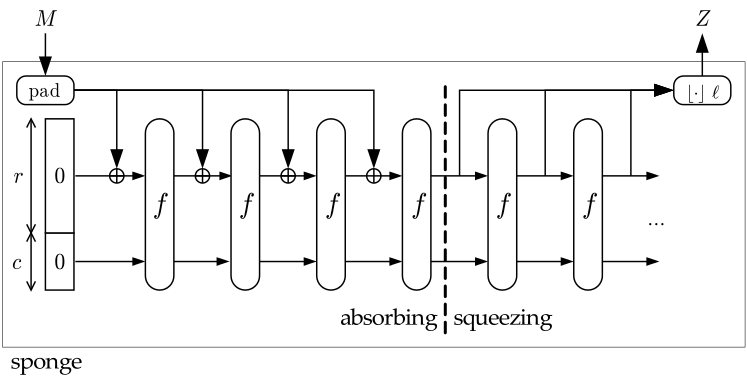
\includegraphics[scale=0.7]{sponge.png}
\caption{Schéma konstrukce \textquote{houby}}
\caption{Zdroj: The sponge and duplex constructions \cite{sponge}}
\label{fig:sponge}
\end{figure}

\subsection{Permutace Keccak-\(f\)}

Jde o~skupinu permutací, které jsou využívány jako transformační funkce na bloky bitů během zpracovávání v~konstrukci sponge. Stav zpracovávání je v~této funkci interpretován jako trojrozměrná matice s~dimenzemi \(5 \times 5 \times w\), kde pro \(w\) platí \(25w = b\). Pro všechny funkce SHA-3 je \(w = 64\), to umožňuje optimální zpracování pro 64-bitové procesory. Obrázek \ref{fig:state} ilustruje jednotlivé komponenty stavové matice. \par

\begin{figure}[ht!]
\centering
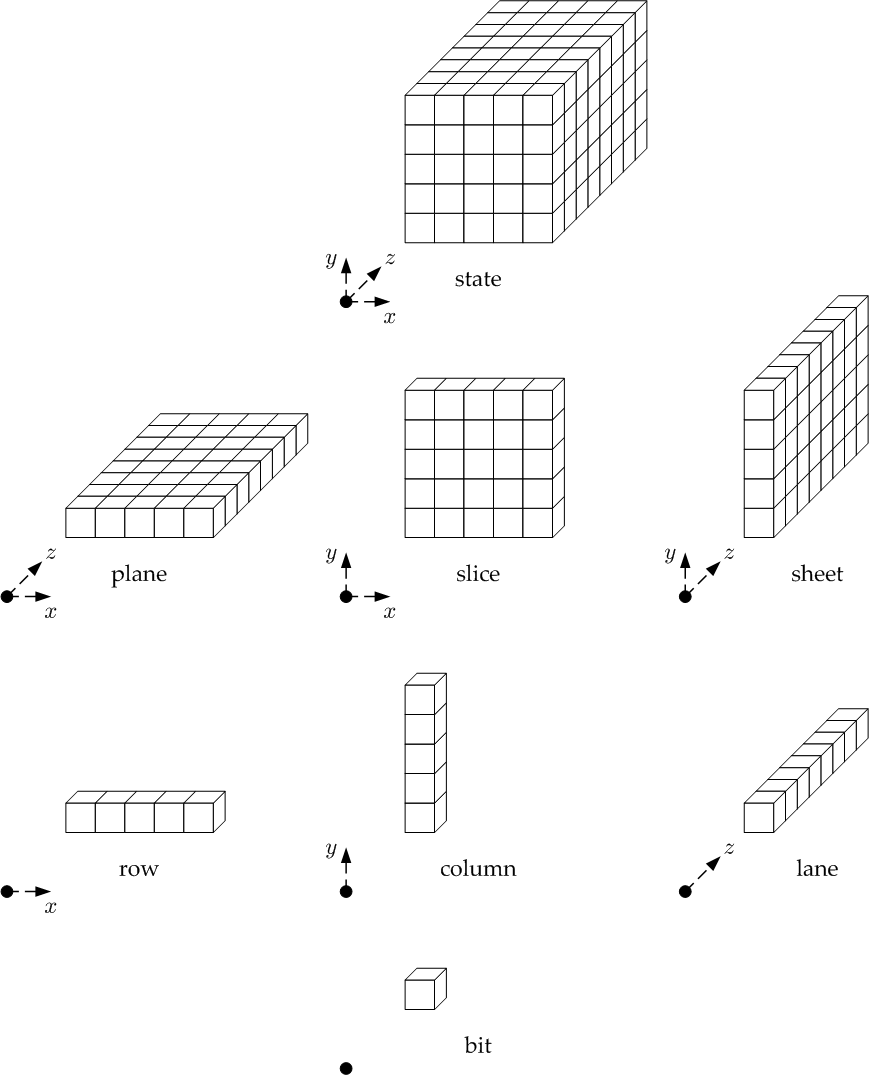
\includegraphics[scale=0.5]{state.png}
\caption{Stavová matice permutací}
\label{fig:state}
\end{figure}

Permutace využívá kromě parametru šířky permutace \(w\) také parametr počet iterací permutace \(n\), který je závislý na šířce vztahem \(n = 12 + 2\log_2(w)\). \par
Jedna iterace se skládá z~pěti kroků.

\begin{enumerate}
    \item \(\theta\) \par
    Tento krok každý bit stavové matice přetransformuje pomocí operace XOR s~paritami dvou sousedních sloupců matice, tak jako na obrázku \ref{fig:theta}.
    
    \item \(\rho\) \par
    Tento krok zrotuje každý bit v~pruhu stavové matice o~počet pozic, který je závislý na souřadnicích tohoto pruhu matice. Operace je vidět na obrázku \ref{fig:rho}.
    
    \item \(\pi\) \par
    Zde jsou přehozeny jednotlivé pruhy matice tak jako na obrázku \ref{fig:pi}.
    
    \item \(\chi\) \par
    Zde je každý bit matice přetransformován operací XOR s~nelineární funkcí dvou sousedních bitů, tak jako na obrázku \ref{fig:chi}.
    
    \item \(\iota\) \par
    Tento krok vyžaduje další parametr zvaný index opakování \(i_r\). Efekt tohoto kroku je, že upraví některé prvního pruhu stavové matice v~závislosti na parametru \(i_r\).
\end{enumerate}


    
\begin{figure}[ht!]
\centering
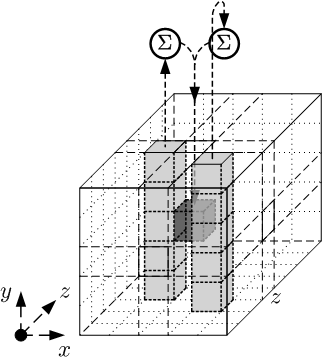
\includegraphics[scale=0.9]{theta.png}
\caption{Schéma prvního kroku permutací Keccak-\(f\)}
\label{fig:theta}
\end{figure}

\begin{figure}[ht!]
\centering
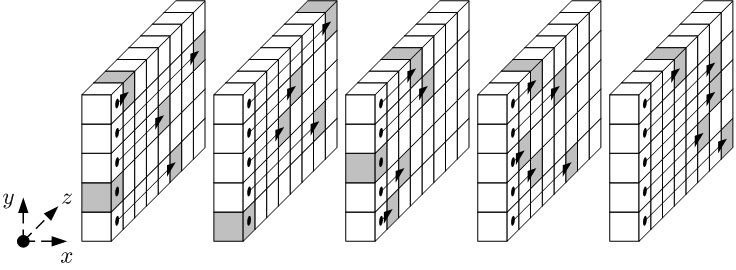
\includegraphics[scale=0.9]{rho.png}
\caption{Schéma kroku \(\rho\) permutací Keccak-\(f\)}
\label{fig:rho}
\end{figure}

\begin{figure}[ht!]
\centering
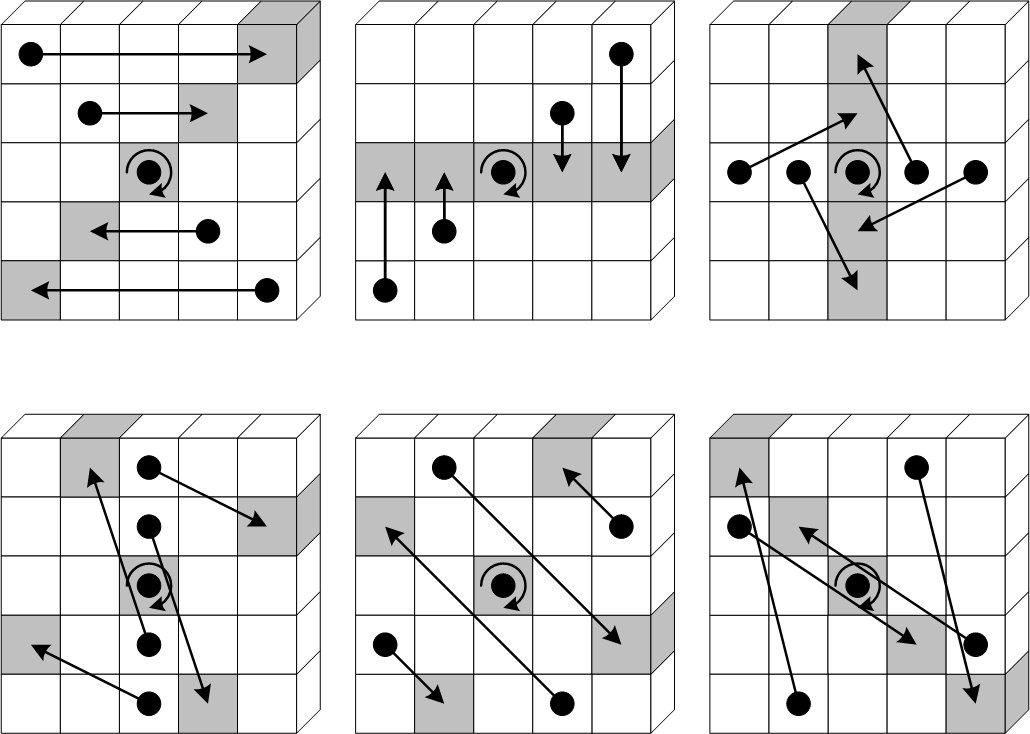
\includegraphics[scale=0.75]{pi.png}
\caption{Schéma kroku \(\pi\) permutací Keccak-\(f\)}
\label{fig:pi}
\end{figure}

\begin{figure}[ht!]
\centering
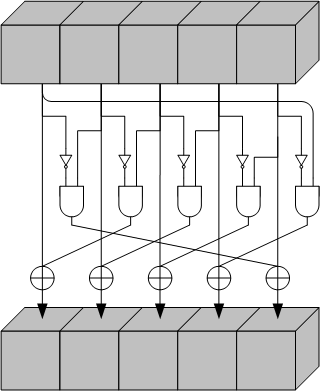
\includegraphics[scale=0.9]{chi.png}
\caption{Schéma kroku \(\chi\) permutací Keccak-\(f\)}
\label{fig:chi}
\end{figure}

\subsection{Padding rule}

Další komponentou algoritmu je takzvané padding rule. To určuje, čím mají být vyplněny bity mezi koncem vstupního bloku a bloku, který je zpracováván uvnitř funkce sponge. Pro funkce SHA-3 je použito takzvané pravidlo \texttt{pad10*1}. To určuje, že všechny zbylé bity budou mít kromě krajních bitů hodnotu 0. 

\section{Popis implementace}

Semestrální práce je implementována v~programovacím jazyce Python~3. Program je rozdělen do dvou modulů.Modul \texttt{sha3.py} obsahuje vstupní bod programu, zpracovává argumenty příkazové řádky a interaguje se vstupními a výstupními soubory. \par
Modul \texttt{keccak.py} obsahuje metody pro výpočet hodnoty hash funkce. Metoda \texttt{keccakRound} obsahuje pět kroků permutace Keccak-\(f\), které daným postupem bitových operací upravují daný pruh matice. Metoda \texttt{keccakF} převádí stav sponge funkce z~bitového řetězce na trojrozměrnou matici, kterou předává ji jako parametr metodě \texttt{keccakRound}, a poté převádí její výsledek zpět na bitový řetězec. Metoda \texttt{keccakSponge} obsahuje hlavní implementaci funkce sponge. Nejprve tedy inicializuje stavovou strukturu, do které postupně v~absorpční fázi uloží vstupní zprávu a přidá na její konec specifické identifikační bity SHA-3 funkcí. Poté voláním předchozích metod upravuje stavovou strukturu, kterou nakonec vrátí jako výstup požadované délky.\par
Na (Listing 1) je ukázán kód metody \texttt{sha3}.

\begin{lstlisting}[caption={Definice metody sha3},captionpos=b]
def sha3(inputBytes, hashLength = 224):
    # check received sha3 length is supported
    validLengths = [224, 256, 384, 512]
    if hashLength not in validLengths:
        raise ValueError("{} is not a supported sha3 length".format(hashLength))
    
    return keccakSponge((hashLength * 2), inputBytes, 0x06, (hashLength // BYTE_SIZE))
\end{lstlisting}

\section{Uživatelská dokumentace}

Ke spuštění programu je zapotřebí mít nainstalován interpret programovacího jazyka Python~3. Program byl testován pro verze Python~3.5 a vyšší. Po rozbalení archivu je možné program spustit příkazem \texttt{python3 sha3.py}. Zde je přehled všech možných voleb, které lze programu předat:

\begin{itemize}
    \item -h \par
    Vypíše na obrazovku zprávu o~možných volbách a jednoduchou nápovědu, poté se ukončí.
    \item -i <inputFile>, --input=<inputFile> \par
    Spustí program v~režimu čtení souboru. Obsah předaného souboru je použit jako vstupní zpráva hashovací funkce.
    \item -o <outputFile>, --output=<outputFile> \par
    Výstup hashovací funkce je místo na obrazovku uložen do souboru.
     \item -l <hashLength>, --length=<hashLength> \par
    Nastaví délku výstupu a podle toho použitý režim hashovací funkce. Podporované jsou délky 224, 256, 384 a 512. Pokud není tato volba uvedena, je nastavena hodnota 224.
\end{itemize}

Pokud není program zapnut v~režimu čtení souboru, použije se jako vstup první argument předaný na příkazové řádce. Pokud na příkazové řádce nebyl předán žádný parametr, je vstup přečten z~proudu standardního vstupu.

\section{Závěr}

Tato práce popisuje rodinu kryptografických funkcí SHA-3, tak jak byla specifikována standardem \cite{dworkin2015sha} Národního institutu pro standardy a technologie USA (NIST). V~tomto dokumentaci je stručně popsáno, co je to kryptografická hashovací funkce, k~čemu ji lze využít a jsou nastíněny principy algoritmu funkcí SHA-3. Vypracovaný program je praktickou ukázkou implementace zmiňovaného standardu. Pro získání referenčních hodnot při kontrole funkčnosti programu byl použit online nástroj \cite{tool}. Získané výstupní hodnoty se shodovaly.

\bibliographystyle{plainnat}
 \bibliography{references}
\end{document}